\documentclass[12pt, a4paper]{article}

% ─── Packages ───────────────────────────────────────────────────────────────
\usepackage[utf8]{inputenc}
\usepackage[T1]{fontenc}
\usepackage[a4paper, top=1in, bottom=1in, left=1.1in, right=1.1in]{geometry}
\usepackage{lmodern}
\usepackage{microtype}
\usepackage{setspace}
\setstretch{1.15}
\usepackage{parskip}
\usepackage{graphicx}
\usepackage{float}
\usepackage[explicit]{titlesec}
\usepackage{fancyhdr}
\usepackage{hyperref}
\usepackage{amsmath}
\usepackage{amssymb}
\usepackage{xcolor}
\usepackage{listings}
\usepackage{tikz}
\usetikzlibrary{shapes.geometric, arrows.meta, positioning, fit, shadows.blur, calc}
\usepackage{booktabs}
\usepackage{tabularx}
\usepackage{enumitem}
\usepackage{tcolorbox}
\tcbuselibrary{skins, breakable}
\usepackage{array}
\usepackage{colortbl}

% ─── Color Palette ──────────────────────────────────────────────────────────
\definecolor{axonpurple}{RGB}{108, 99, 255}
\definecolor{axondark}{RGB}{24, 24, 37}
\definecolor{axongray}{RGB}{240, 240, 245}
\definecolor{codegreen}{RGB}{40, 160, 40}
\definecolor{axongold}{RGB}{198, 138, 0}

% ─── Hyperref Configuration ──────────────────────────────────────────────────
\hypersetup{
    colorlinks=true,
    linkcolor=axonpurple,
    urlcolor=axonpurple!80!black,
    pdftitle={Axon Flow: Product Pitch},
    pdfauthor={Akshat Raj \& Pavan Soni}
}

% ─── Section Styling ─────────────────────────────────────────────────────────
\titleformat{\section}{\Large\bfseries\color{axonpurple}}{}{0em}
  {\colorbox{axonpurple!10}{\parbox{\dimexpr\linewidth-2\fboxsep}{\thesection\quad #1}}}
\titleformat{\subsection}{\large\bfseries\color{axondark!90}}{}{0em}{\thesubsection\quad #1}
\titleformat{\subsubsection}{\normalsize\bfseries}{}{0em}{\thesubsubsection\quad #1}

% ─── Header / Footer ─────────────────────────────────────────────────────────
\pagestyle{fancy}
\fancyhf{}
\fancyhead[L]{\textcolor{axonpurple}{\textbf{Axon Flow}} | Product Pitch}
\fancyhead[R]{\leftmark}
\fancyfoot[R]{\thepage}
\renewcommand{\headrulewidth}{0.5pt}
\renewcommand{\footrulewidth}{0pt}
\addtolength{\headheight}{2.5pt}

% ─── Custom Commands ────────────────────────────────────────────────────────
\newtcolorbox{callout}[1][]{
  colback=axonpurple!5,
  colframe=axonpurple!80,
  left=12pt,
  right=12pt,
  top=8pt,
  bottom=8pt,
  sharp corners,
  boxrule=0.8pt,
  leftrule=4pt,
  enhanced,
  #1
}

\newtcolorbox{questionbox}[1][]{
  enhanced, breakable, colback=axonpurple!5, colframe=axonpurple!80,
  title=#1, fonttitle=\bfseries\large, coltitle=white,
  left=10pt, right=10pt, top=10pt, bottom=10pt
}

\newtcolorbox{answerbox}[1][]{
  enhanced, breakable, colback=black!2, colframe=black!30,
  title=#1, fonttitle=\bfseries\large, coltitle=black,
  left=10pt, right=10pt, top=10pt, bottom=10pt
}

% ════════════════════════════════════════════════════════════════════════════
\begin{document}
\pagenumbering{gobble}

% ─── Title/Cover Page ───────────────────────────────────────────────────────
\begin{titlepage}
  \centering
  \vspace*{1.5cm}
  
  % Logo Visualized with TikZ
  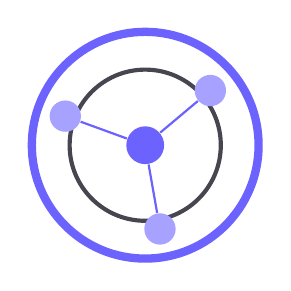
\begin{tikzpicture}[scale=1.2, every node/.style={transform shape}]
    \draw[line width=3pt, axonpurple] (0,0) circle (1.2cm);
    \draw[line width=1.5pt, axondark!80] (0,0) circle (0.8cm);
    
    \node[circle, fill=axonpurple, minimum size=0.4cm] (c) at (0,0) {};
    
    \node[circle, fill=axonpurple!60, minimum size=0.25cm] (n1) at (40:0.9cm) {};
    \node[circle, fill=axonpurple!60, minimum size=0.25cm] (n2) at (160:0.9cm) {};
    \node[circle, fill=axonpurple!60, minimum size=0.25cm] (n3) at (280:0.9cm) {};
    
    \draw[thick, axonpurple] (c) -- (n1);
    \draw[thick, axonpurple] (c) -- (n2);
    \draw[thick, axonpurple] (c) -- (n3);
  \end{tikzpicture}
  
  \vspace{1.5cm}
  {\Huge\bfseries\color{axondark} AXON FLOW\par}
  \vspace{0.4cm}
  {\large\bfseries\color{axonpurple} A Performant, Browser-Native Mind-Mapping Platform\\with Client-Side D3 Geometry and Optimistic UI\par}
  
  \vspace{1.0cm}
  \rule{\textwidth}{1pt}
  \vspace{1.0cm}
  
  \begin{minipage}[t]{0.45\textwidth}
    \centering
    \textbf{Prepared By:}\\
    Akshat Raj\\
    {\small (Reg. No: 23scse1010833)}
  \end{minipage}
  \begin{minipage}[t]{0.45\textwidth}
    \centering
    \textbf{Collaborator:}\\
    Pavan Soni\\
    {\small (Reg. No: 23scse1012576)}
  \end{minipage}
  
  \vspace{1.5cm}
  \textbf{Institution:}\\
  Department of Computer Science \& Engineering\\
  Galgotias University\\
  Greater Noida, India
  
  \vfill
  {\large\today\par}
\end{titlepage}

\newpage
\pagenumbering{arabic}

% ─── Section 1: Executive Summary ───────────────────────────────────────────
\section{Executive Summary}

Brainstorming and knowledge mapping tools have transitioned from analog whiteboards to critical collaborative software. However, existing modern platforms (such as Miro, XMind, and GitMind) suffer from performance limitations, severe interface latency, and security concerns from pushing private brainstorming data into cloud AI clusters.

\textbf{Axon Flow} solves these problems by decoupling data representation from rendering layout. By combining a flat independent node model with local D3-Hierarchy calculations and an instantaneous Optimistic UI feedback loop, Axon Flow delivers a desktop-grade, zero-latency collaborative canvas running entirely in a standard browser. Additionally, it integrates a local, private Generative AI engine that runs offline, ensuring user data privacy.

\subsection{What is Axon Flow? (Non-Technical Key Points)}
To introduce the project in simple, clear terms, here are the core concepts:
\begin{itemize}[label=\small$\bullet$, leftmargin=15pt]
  \item \textbf{Infinite Digital Notebook:} Axon Flow is an interactive web-based mind map where users can brainstorm and connect ideas visually on an infinite canvas.
  \item \textbf{Instant UI Updates:} Unlike other tools that freeze or show loading spinners on every change, Axon Flow updates the screen instantly (0ms delay) and saves changes silently in the background.
  \item \textbf{Text and Mind-Map Dual View:} It bridges the gap between visual diagrams and linear reading by allowing users to toggle their maps into structured text outlines (like a reading tutorial).
  \item \textbf{Local, Secure AI:} Users can ask the built-in AI assistant to auto-expand branches or outline topics offline, keeping their brainstorming private.
  \item \textbf{Unified Study Hub:} Each node on the map acts as a repository where users can store Markdown notes, status indicators, hyperlinks, and upload reference files.
\end{itemize}

\begin{callout}[title=\textbf{Value Proposition}]
  Axon Flow offers an \textbf{instantaneous (0ms perceived latency)} visual mind-mapping canvas that handles over 500 nodes at 60 FPS, features a linearized reading mode to prevent canvas fatigue, and maintains strict user privacy with local LLM capabilities.
\end{callout}

% ─── Section 2: Market Pain Points & The Problem ────────────────────────────
\section{Market Pain Points \& The Problem}

Modern digital mind-mapping tools exhibit three core bottlenecks that hinder productivity:

\begin{enumerate}[leftmargin=*, label=\textbf{\arabic*.}]
  \item \textbf{Nested-Document Database Overheads}: Standard tools store entire mind-map trees as a single nested document (JSON) in the database. When a user updates, moves, or renames a single node, the entire hierarchy must be sent over the network and rewritten in the database. This leads to heavy database lock times, write-amplification, and synchronization conflicts in multi-user settings.
  
  \item \textbf{Canvas Fatigue and Layout Disorientation}: As a mind-map grows beyond 50 nodes, users suffer from "canvas fatigue." Continuously panning and zooming to read notes or edit leaf structures becomes disorienting. Traditional tools fail to offer a cohesive way to consume deep visual structures linearly.
  
  \item \textbf{Heavy DOM Rendering and UI Latency}: Tools that render canvas bubbles using hundreds of nested HTML \texttt{div} tags trigger browser reflows and layout recalculations on every drag event. This degrades frame rates (<15 FPS) and introduces noticeable lag. Alternatively, server-side layouts introduce a delay (200ms–1.5s) on every user action while waiting for the database confirmation.
\end{enumerate}

\newpage

% ─── Section 3: Technical Solution & Innovation ─────────────────────────────
\section{Technical Solution \& Innovation}

Axon Flow solves these fundamental constraints with a modern, high-performance architecture:

\subsection{Flat-Tree Data Model}
Rather than nested JSON documents, every node in Axon Flow is an independent document in MongoDB. The document tracks only three primary keys: `id`, `mapId`, and `parentId`. 
$$\text{Update Complexity: } O(1) \text{ database update query}$$
Updating a node's name, content, or collapsing a branch modifies only that single record via a lightweight \texttt{PATCH} request, avoiding database write-amplification.

\subsection{Client-Side D3 Geometry calculations}
The server acts as a lightweight data dispenser, sending a flat list of nodes to the client. The frontend then reconstructs the visual tree in memory using \texttt{D3-Hierarchy}'s layout stratify algorithms in under \textbf{1 millisecond} for 500 nodes. Nodes are positioned dynamically based on label width calculations.

\subsection{Zero-Latency Optimistic UI}
Axon Flow updates the UI state instantly based on expected success. When a node is added, renamed, or reparented via drag-and-drop:
\begin{enumerate}[label=\alph*)]
  \item The local React state is updated immediately (0ms delay).
  \item D3 math computes coordinates in the background.
  \item A silent network request is dispatched.
  \item If the request fails, the local state is rolled back and the user is notified.
\end{enumerate}

% ─── Section 4: Product Features & Functionality ───────────────────────────
\section{Product Features \& Functionality}

\begin{itemize}[leftmargin=*]
  \item \textbf{Document-Wise Reading Mode}: Toggles the visual layout into a structured text document. The D3 visual tree is linearized into hierarchical headings (H1, H2, H3) based on depth, displaying markdown notes and code attachments inline. This eliminates panning and zoom fatigue.
  
  \item \textbf{Radial Status Indicators}: Visual toggle pins on each node allow students and developers to track learning/completion states (\textit{Reading, Completed, Revising, Important}) directly from the canvas or the outline view.
  
  \item \textbf{Offline Local AI Assistant}: A FastAPI service utilizing Ollama and LangChain streams AI topics (SSE protocol) to automatically expand node trees based on prompt topics, operating strictly on the user's local machine for absolute data privacy.
\end{itemize}

\newpage

% ─── Section 5: The User Journey & Non-Technical Modules ──────────────────────
\section{The User Journey \& Non-Technical Modules}

To understand how Axon Flow works in practice, let us look at the platform through a universal user workflow of building, enriching, and utilizing a mind map:

\subsection{The Universal User Workflow}
\begin{enumerate}[leftmargin=*, label=\textbf{\alph*)}]
  \item \textbf{Instant Brainstorming (The Map Canvas):}
    \begin{itemize}[label=\small$\bullet$, leftmargin=15pt]
      \item The user opens Axon Flow and is presented with a clean, \textbf{infinite digital canvas}.
      \item With a simple \textbf{double-click}, a new node bubble is created instantly on the workspace with \textbf{zero network delay (0ms)}.
      \item The user types a topic label, and the bubbles automatically slide apart mathematically to maintain neat coordinates.
    \end{itemize}
    
  \item \textbf{Creating Nodes, Adding Files \& Resource Links:}
    \begin{itemize}[label=\small$\bullet$, leftmargin=15pt]
      \item The user creates child branches and \textbf{uploads reference PDFs, slides, or code files} directly to any node.
      \item The user embeds \textbf{external hyperlinks} (such as project repositories or online videos) directly inside a node's detail panel.
      \item Rich \textbf{Markdown notes} are typed in the inline text sidebar, consolidating all media resources in one visual hub.
    \end{itemize}

  \item \textbf{AI-Powered Node Expansion:}
    \begin{itemize}[label=\small$\bullet$, leftmargin=15pt]
      \item To automatically expand a concept, the user right-clicks a node and triggers the \textbf{local AI assistant}.
      \item An \textbf{offline Llama 3 model} running locally on the user's laptop brainstorms 4--6 relevant subtopics as children.
      \item These branches sprout instantly on the canvas, keeping the user's proprietary notes \textbf{100\% private and secure}.
    \end{itemize}

  \item \textbf{Linearized Outline Mode (Eliminating Canvas Fatigue):}
    \begin{itemize}[label=\small$\bullet$, leftmargin=15pt]
      \item When the visual canvas becomes too crowded to easily read, the user toggles the \textbf{Document-Wise Reading View}.
      \item The hierarchical D3 visual structure is instantly flattened into \textbf{sequentially organized text headings} (H1, H2, H3).
      \item Notes, file attachments, and code snippets render inline, reading naturally like a \textbf{digital notebook chapter}.
    \end{itemize}

  \item \textbf{Interactive Progress Tracking (Radial Status Badges):}
    \begin{itemize}[label=\small$\bullet$, leftmargin=15pt]
      \item Next to each header or node bubble, the user selects a \textbf{radial button} to update their study or task state.
      \item The user toggles status badges across states such as \textbf{\textit{Completed} ($\checkmark$)}, \textbf{\textit{Reading} (R)}, or \textbf{\textit{Revising} (!)}.
      \item Status changes sync instantly in the background, updating both the visual canvas and document outlines simultaneously.
    \end{itemize}
\end{enumerate}

\subsection{Non-Technical Core Modules}
Under the hood, Axon Flow is split into four simple user-facing modules:
\begin{itemize}[leftmargin=*]
  \item[\textcolor{axonpurple}{\tiny$\blacksquare$}] \textbf{The Infinite Creative Canvas:} A drag-and-drop workspace where ideas can be \textbf{visually structured, linked, and organized} without bounds.
  \item[\textcolor{axonpurple}{\tiny$\blacksquare$}] \textbf{The Smart Reader (Document Mode):} A linearized text workspace that turns visual diagrams into \textbf{organized outline guides} with inline attachments.
  \item[\textcolor{axonpurple}{\tiny$\blacksquare$}] \textbf{The Private AI Brainstormer:} A local copilot that helps flesh out subtopics and \textbf{auto-generate mind maps offline} without cloud risks.
  \item[\textcolor{axonpurple}{\tiny$\blacksquare$}] \textbf{The Study \& Resource Vault:} A hub attached to every node where \textbf{files, hyperlinks, and status badges} are securely stored.
\end{itemize}

\newpage

% ─── Section 6: Competitive Matrix ──────────────────────────────────────────
\section{Competitive Matrix}

The following table highlights how Axon Flow compares to the leading products in the market:

\begin{table}[H]
  \centering
  \small
  \renewcommand{\arraystretch}{1.3}
  \begin{tabularx}{\textwidth}{l >{\raggedright\arraybackslash}X >{\raggedright\arraybackslash}X}
    \toprule
    \textbf{Dimension} & \textbf{Traditional Tools (Miro/XMind)} & \textbf{Axon Flow} \\
    \midrule
    \rowcolor{axonpurple!5}
    \textbf{Data Privacy} & High risk; data uploaded to cloud LLMs (OpenAI/Anthropic). & \textbf{100\% private}; runs local model offline via Ollama. \\
    
    \textbf{Code Integrations} & Plain text only; no developer attachment capability. & Bind \textbf{source code, attachments}, and links to nodes. \\
    
    \rowcolor{axonpurple!5}
    \textbf{Reading Experience} & Panning/zooming fatigue on deep visual maps. & Dual view: Switch to linear \textbf{Document-Wise Outlines}. \\
    
    \textbf{UI Performance} & Heavy canvas redraws causing lag during drags. & Flat MongoDB schema + React Virtual DOM translation. \\
    
    \rowcolor{axonpurple!5}
    \textbf{Perceived Latency} & 200ms--1.5s (blocking network spinners). & \textbf{0ms (Optimistic UI background syncing)}. \\
    \bottomrule
  \end{tabularx}
  \caption{Product Comparison Matrix}
  \label{tab:comparison}
\end{table}

% ─── Section 7: Architecture & Implementation Plan ─────────────────────────
\section{Architecture \& Implementation Plan}

Axon Flow is designed around the \textbf{"Smart Client, Dumb Server"} paradigm. The backend (Node.js/Express) serves only to store independent relational records, validate tokens via Clerk, and handle file attachments in S3. 

\begin{figure}[H]
  \centering
  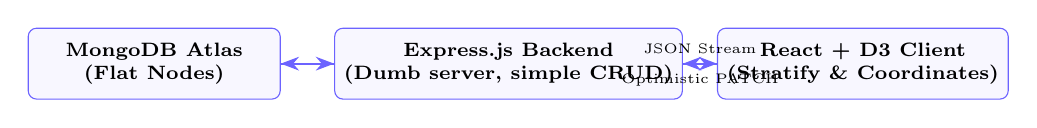
\begin{tikzpicture}[
    box/.style={rectangle, draw=axonpurple, fill=axonpurple!5, rounded corners=3pt, minimum width=3.2cm, minimum height=0.9cm, align=center, font=\scriptsize\bfseries},
    arrow/.style={-Stealth, thick, draw=axonpurple}
  ]
    \node[box] (db) at (0,0) {MongoDB Atlas\\(Flat Nodes)};
    \node[box] (api) at (4.5,0) {Express.js Backend\\(Dumb server, simple CRUD)};
    \node[box] (client) at (9.0,0) {React + D3 Client\\(Stratify \& Coordinates)};
    
    \draw[arrow] (api) -- node[above, font=\tiny]{JSON Stream} (client);
    \draw[arrow] (client) -- node[below, font=\tiny]{Optimistic PATCH} (api);
    \draw[arrow] (api) -- (db);
    \draw[arrow] (db) -- (api);
  \end{tikzpicture}
  \caption{Data Flow Architecture}
  \label{fig:data_flow}
\end{figure}

The project is structured for a three-phase rollout:
\begin{itemize}[label=\checkmark]
  \item \textbf{Phase 1 (Core Canvas)}: Client-side layout parsing and flat schema updates.
  \item \textbf{Phase 2 (Optimistic UI \& Files)}: Implementation of drag-and-drop hit tests, offline rollbacks, and file uploads.
  \item \textbf{Phase 3 (Local AI \& Stream)}: FastAPI integration with local Ollama SSE stream nodes.
\end{itemize}

% ─── Section 8: Project Key Points & Quick Summary ──────────────────────────
\newpage
\section{Project Key Points \& Quick Summary}

\subsection{About My Project}
\begin{itemize}[label=\small$\bullet$, leftmargin=15pt, nosep]
  \item Performant browser-native mind mapper
  \item Decentralized flat-data structure model
  \item High-speed mathematical client layout
  \item Server-Sent Events (SSE) token generator
  \item Zero-latency optimistic canvas updates
  \item Offline local LLM expansion
  \item Linearized reading dual outlines
\end{itemize}

\subsection{Key Features}
\begin{itemize}[label=\small$\bullet$, leftmargin=15pt, nosep]
  \item \textbf{0 Perceived Latency:} Predictive local node updates
  \item \textbf{Optimistic State Sync:} Background Mongo saves with rollback protection
  \item \textbf{Sub-millisecond D3 Stratification:} In-memory JSON tree rebuilding
  \item \textbf{Linearized Outline Mode:} Flat heading outlining (H1, H2, H3)
  \item \textbf{Offline Local Copilot:} Topic expansion using Ollama models
  \item \textbf{SSE Typewriter Stream:} Unidirectional chunk-by-chunk token push
  \item \textbf{Visual Status Badging:} Task indicators ($\checkmark$, Reading, Revision, Important)
  \item \textbf{Media Node Vault:} PDF uploads, custom hyperlinks, notes attachments
  \item \textbf{Native Drag/Resize Listeners:} Lightweight mouse listeners
  \item \textbf{Microservices Auth Gateway:} Clerk-integrated backend checks
\end{itemize}

\subsection{Core Modules}
\begin{itemize}[label=\small$\bullet$, leftmargin=15pt, nosep]
  \item \textbf{Infinite Creative Canvas:} SVG coordinate dragging and layout grid
  \item \textbf{Smart Outline Reader:} Monolithic map linearized outline guide
  \item \textbf{Offline AI Brainstormer:} Direct LLM inference node stream
  \item \textbf{Resource Repository:} File and link storage per node
  \item \textbf{Authentication Gateway:} Node.js request router and token check
  \item \textbf{Business Core Engine:} Spring Boot MVC backend
\end{itemize}

\subsection{Technology Stack}
\begin{itemize}[label=\small$\bullet$, leftmargin=15pt, nosep]
  \item \textbf{Frontend Base:} React, Vite, ES6 JS
  \item \textbf{UI Canvas Layout:} React Flow
  \item \textbf{Layout Math Brain:} D3-Hierarchy (tree, stratify)
  \item \textbf{Gateway Route Manager:} Node.js, Express, JWT
  \item \textbf{Core Persistence Service:} Java, Spring Boot, Spring Data MongoDB
  \item \textbf{Database Storage System:} MongoDB Atlas
  \item \textbf{AI Execution Runtime:} Python, FastAPI, EventSource API
  \item \textbf{AI Orchestration Framework:} LangChain, Ollama Client
  \item \textbf{Local AI Models:} Llama 3 / DeepSeek R1
  \item \textbf{File Storage Space:} S3 / Local Disk
\end{itemize}

\subsection{Why This Project? (Motivation)}
\begin{itemize}[label=\small$\bullet$, leftmargin=15pt, nosep]
  \item \textbf{Prevent AI Cloud Leaks:} Keep sensitive client mapping data offline
  \item \textbf{Solve Nested JSON Locks:} Flat collection maps avoid monolithic writes
  \item \textbf{Solve Canvas Repaint Lags:} SVG layout calculation renders 500+ nodes at 60 FPS
  \item \textbf{Prevent Pan/Zoom Canvas Fatigue:} Quick conversion to outlines
  \item \textbf{Deliver Seamless Latency-Free UX:} Ghost nodes remove load spinners
  \item \textbf{Master Polyglot Microservices:} Combine Spring, Node, Python architectures
\end{itemize}

% ─── Section 9: Project Quick Reference & Learning Guide ──────────────────
\newpage
\section{Project Quick Reference \& Learning Guide}

To assist in understanding, defending, and discussing the technical architecture of Axon Flow, the key concepts, features, and engineering challenges are summarized below keyword-wise.

\subsection{Core Project Concepts \& Architecture (Keyword-Wise)}
\begin{itemize}[leftmargin=*]
  \item \textbf{Polyglot Microservices Topology:} The architecture decouples tasks across different runtimes matching specific computational bounds:
    \begin{itemize}
      \item \textit{Frontend (React + Vite):} Renders the interactive UI and computes layout geometry.
      \item \textit{Backend (Spring Boot + MongoDB):} Manages database transactions, permissions, and node relational persistence.
      \item \textit{AI Engine (FastAPI + Python):} Orchestrates local LLM inference, LangChain tools, and SSE streaming.
    \end{itemize}
  \item \textbf{I/O Gateway vs. CPU Processing:} Node.js handles I/O-bound API routing (Gateway) via its single-threaded non-blocking event loop, whereas Spring Boot handles transactional integrity, and Python handles CPU/GPU-bound local LLM inference.
  \item \textbf{Flat-Tree Schema Representation:} Relational node records are stored flat in MongoDB via \texttt{\{id, parentId, mapId\}}, preventing write amplification, database locks, and sync conflicts common in monolithic JSON trees.
  \item \textbf{Data Driven Document (D3) Geometry:} The client calculates mathematical coordinate layouts in-memory using D3-Hierarchy (\texttt{d3.stratify()} and \texttt{d3.tree()}) in under 1ms, decoupling layout computation from DOM rendering.
\end{itemize}

\subsection{Key Product Features (Keyword-Wise)}
\begin{itemize}[leftmargin=*]
  \item \textbf{Optimistic UI Synchronization:} Updates local React state instantly to render node operations, running coordinate layouts in the background and syncing via background network requests (0ms perceived latency).
  \item \textbf{Linearized Document-Wise Outlines:} Translates the two-dimensional D3 canvas nodes into hierarchical text outlines (H1, H2, H3) inline with rich-text Markdown notes, eliminating canvas pan/zoom fatigue.
  \item \textbf{Offline Local AI Assistant:} Auto-generates and expands concept trees using local LLMs (via Ollama) running offline on the user's system, guaranteeing absolute privacy.
  \item \textbf{Server-Sent Events (SSE):} Streams AI-generated tokens to the client character-by-character, preventing blocking page loads and displaying live, typewriter-like thinking text.
  \item \textbf{Radial Status Badge Controls:} Interactive visual indicators (\textit{Reading, Completed, Revising, Important}) that sync in real time between the visual canvas and linear document outlines.
\end{itemize}

\subsection{Technical Challenges \& Solutions (Keyword-Wise)}
\begin{itemize}[leftmargin=*]
  \item \textbf{Challenge: Nested JSON Serialization Failures (Jackson Serialization)}
    \begin{itemize}
      \item \textit{Problem:} Dynamic node metadata (like lists of links and files) failed to deserialize properly at the Spring Boot backend, collapsing to generic objects or causing null values.
      \item \textit{Solution:} Changed the Java persistence entity field structure to \texttt{List<Map<String, Object>>} with explicit null-guard setters to ensure type safety.
    \end{itemize}
  \item \textbf{Challenge: Broken JSON from Local LLMs (JSON Extraction)}
    \begin{itemize}
      \item \textit{Problem:} Smaller offline models (like Llama 3) frequently emit incomplete JSON blocks or surround response streams in markdown wrappers, breaking frontend parsers.
      \item \textit{Solution:} Developed a multi-stage parser in the Python AI Engine using regular expressions, curly brace counting, and automated repairs to sanitize and parse malformed streams.
    \end{itemize}
  \item \textbf{Challenge: Heavy DOM Reflows during Canvas Dragging (UI Lag)}
    \begin{itemize}
      \item \textit{Problem:} Redrawing coordinate connections and updating node elements using standard React state updates triggers browser paint/reflow loops, dropping frame rates.
      \item \textit{Solution:} Integrated native D3 geometry math to run calculations in-memory, updating coordinates directly via SVG properties while leaving the React Virtual DOM unaffected.
    \end{itemize}
  \item \textbf{Challenge: Drag-and-Drop Library Bloat}
    \begin{itemize}
      \item \textit{Problem:} Importing third-party canvas libraries (e.g. react-dnd) increases bundle size and introduces unnecessary configuration overhead.
      \item \textit{Solution:} Implemented a native mouse event listener (\texttt{mousedown, mousemove, mouseup}) bound to the window to calculate delta coordinates.
    \end{itemize}
\end{itemize}

\newpage
% ─── Section 10: Interview Questions & Answers ──────────────────────────────
\section{Interview Questions \& Answers}

\begin{questionbox}[Question 1: D3 vs React Flow]
For making a deep nested hierarchy, is this step a must (like using D3 inside the pipeline)? Or is there any shortcut in React Flow?
\end{questionbox}

\begin{answerbox}[Answer]
\textbf{Yes, using an external layout engine like D3 (or Dagre/ELK) is completely necessary.} React Flow does not support automatic hierarchical layout calculations out-of-the-box.
\begin{itemize}
  \item \textbf{React Flow is a Dumb Canvas:} React Flow only physicalizes nodes on a coordinate grid. If coordinates are not provided, all nodes pile up at $(0,0)$. It lacks tree layout calculation logic.
  \item \textbf{D3-Hierarchy is the Brains:} We use D3 to construct the nested hierarchy in-memory (\texttt{d3.stratify()}) and run advanced node spacing algorithms (\texttt{d3.tree()}) to calculate perfect non-overlapping coordinates.
\end{itemize}
\end{answerbox}

\begin{questionbox}[Question 2: Polyglot Microservices Selection]
Why did you choose a Polyglot Microservices architecture (Node.js API Gateway, Java/Spring Boot Core Backend, and Python FastAPI AI Engine) instead of a monolithic single-language setup?
\end{questionbox}

\begin{answerbox}[Answer]
This structure aligns each service with its exact computational profile, ensuring optimal performance:
\begin{itemize}
  \item \textbf{Node.js API Gateway (I/O Bound):} Handles concurrent connection routing and token verification. Its non-blocking, single-threaded event loop handles high request volumes with low memory footprint.
  \item \textbf{Java/Spring Boot Core Backend (Logic Bound):} Handles hierarchical operations and relational persistence. Java's strong typing, OOP design, and robust transaction management ensure structural integrity.
  \item \textbf{Python FastAPI AI Engine (CPU/GPU Bound):} Handles LLM prompt construction, agent workflows, and token parsing. Python is the industry standard for AI, and FastAPI supports asynchronous SSE streaming out-of-the-box.
\end{itemize}
\end{answerbox}

\begin{questionbox}[Question 3: Google Login (OAuth2) Flow]
How does Google Login (OAuth2) authentication work in this polyglot microservice architecture, and how do you handle tokens?
\end{questionbox}

\begin{answerbox}[Answer]
We use Google as an identity validator, but manage API security via a custom system token:
\begin{itemize}
  \item \textbf{Step 1 (Google Token):} React logs in via Google and receives a short-lived \textbf{Google ID Token}.
  \item \textbf{Step 2 (Verification):} React sends the token through the Node Gateway to Spring Boot. Spring Boot uses \texttt{GoogleIdTokenVerifier} to confirm its authenticity.
  \item \textbf{Step 3 (App JWT):} If valid, Spring Boot registers the user in MongoDB, discards the Google Token, and generates a signed custom \textbf{App JWT}.
  \item \textbf{Step 4 (Subsequent Requests):} React stores the App JWT and sends it in the Authorization header. The Node Gateway validates this App JWT locally for all microservice routing.
\end{itemize}
\end{answerbox}

\begin{questionbox}[Question 5: Client-Side Layout \& Optimistic UI]
How do you optimize canvas rendering performance and minimize perceived layout latency on the client side?
\end{questionbox}

\begin{answerbox}[Answer]
We eliminate lag through decoupled math rendering and predictive state updates:
\begin{itemize}
  \item \textbf{Decoupled Calculations:} Layout math runs programmatically in D3 based on text-label width calculations, completely independent of the DOM paint pipeline.
  \item \textbf{Optimistic State Updates:} The UI updates and draws coordinates instantly upon node insertion, deletion, or moves. The network request is made in the background, rolling back state only on server errors.
\end{itemize}
\end{answerbox}

\begin{questionbox}[Question 6: Software Engineering Principles Alignment]
How does the Axon Flow codebase align with modularity, Single Responsibility Principle (SRP), and clean code guidelines?
\end{questionbox}

\begin{answerbox}[Answer]
The codebase is structured around strict separation of concerns to support scalability:
\begin{itemize}
  \item \textbf{Modularity:} Adheres to Controller-Service-Repository patterns in Spring Boot and keeps UI widgets separated from state-management services in React.
  \item \textbf{Single Responsibility (SRP):} Layout geometry is isolated from React rendering; API operations are abstracted into custom hooks; and LLM parsing logic is handled strictly by Python's helper scripts.
  \item \textbf{Clean Code:} Clutter is reduced by moving inline CSS elements to external stylesheets and refactoring large rendering files into smaller, reusable UI blocks.
\end{itemize}
\end{answerbox}

\newpage
% ─── Section 11: Conclusion ──────────────────────────────────────────────────
\section{Conclusion}

Axon Flow redefines web-based brain-mapping by utilizing client-side computing power. By eliminating blocking network spinners and nested storage patterns, it brings native-level desktop responsiveness directly to the browser, while respecting modern data privacy mandates through local generative models.

\end{document}

